% Created 2011-05-04 Wed 21:11
\documentclass[11pt]{article}
\usepackage[utf8]{inputenc}
\usepackage[T1]{fontenc}
\usepackage{graphicx}
\usepackage{longtable}
\usepackage{float}
\usepackage{wrapfig}
\usepackage{soul}
\usepackage{amssymb}
\usepackage{hyperref}
\usepackage[spanish]{babel}
\usepackage{bookman}
\usepackage[left=2cm,top=3cm,right=2cm,bottom=1cm,head=1.5cm,includefoot]{geometry}
\usepackage{listings}
\usepackage{multirow}
\usepackage{amssymb}
\usepackage{fancyhdr}
\usepackage{comment}
\usepackage{color}
\usepackage{multicol}
\usepackage[table]{xcolor}
\usepackage{ulem}
\usepackage{pdfpages}

\title{Informe}
\author{}
\date{03 Junio 2011}

\begin{document}
%Caratula
\thispagestyle{empty}
  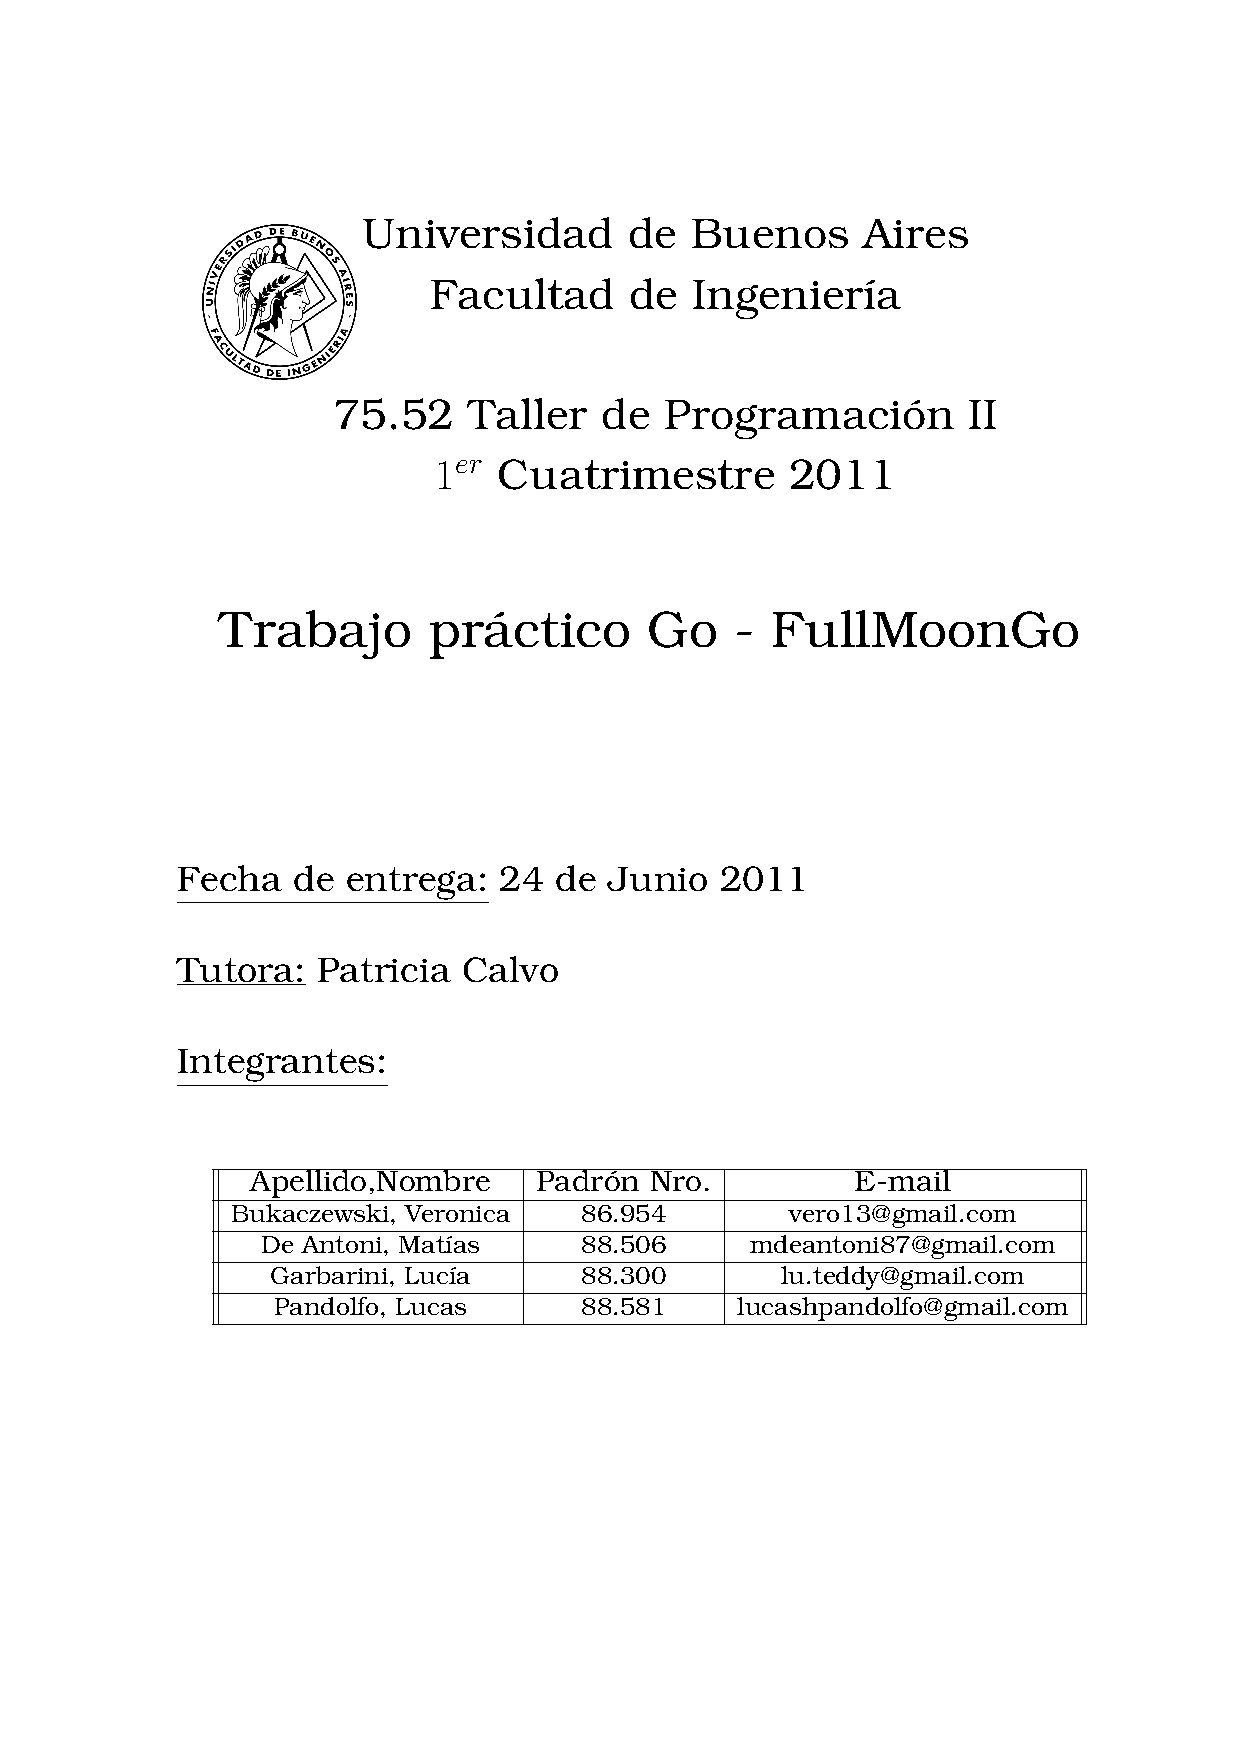
\includepdf[pages=1]{Caratula/Caratula.pdf}

\setcounter{tocdepth}{3}
\tableofcontents

\newpage
\section{Objetivo}
\label{sec-1}

  Desarrollar un sistema que permita jugar partidas de \textbf{Go}, en un
  tablero reducido y considerando el juego finalizado \textbf{a la primera   muerte} (\emph{capture Go}).

\section{Requerimientos funcionales}
\label{sec-2}

  El sistema debe permitir a dos jugadores humanos en la misma
  computadora jugar entre si. También debe permitir como posibles
  participantes del juego a alguna aplicación externa (como ser
  \textbf{gnugo}). Adicionalmente se deben incluir estrategias de juego para
  que una sola persona pueda desarrollar una partida contra el
  sistema.

\section{Manual de usuario}
\label{sec-3}
\underline{Men\'u de inicio}
\begin{center}
 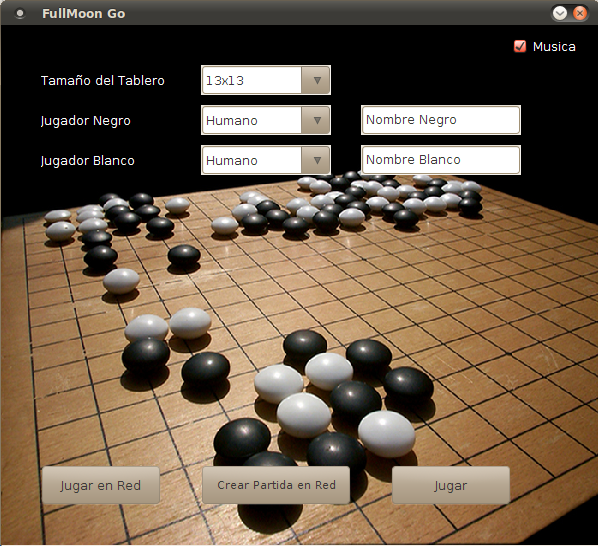
\includegraphics[scale=0.55]{./Diagramas/captura_fullmoon.png}
\end{center}

En el men\'u de inicio se modifica el tama\~no del tablero para jugar, las estrategias de cada jugador y el nombre de cada jugador.
Para jugar una partida local, luego de seleccionar el tablero y los jugadores, se debe presionar el bot\'on ``Jugar''. Si la estrategia
elegida es ``Humano'', las piedras deben ubicarse en el tablero haciendo click con el bot\'on izquierdo del mouse. \\
Para jugar una partida en red, uno de los jugadores debe crear un servidor mediante el bot\'on ``Crear Partida'' donde se pide
el puerto por el cual esperar una conexi\'on. El cliente luego puede unirse mediante el bot\'on ``Jugar en Red'' especificando
la ip y el puerto del servidor.\\ 
Al jugar en red, el cliente juega con el color negro y el servidor con el color blanco, y es el cliente quien decide
el tama\~no del tablero con el cual jugar.\\


\underline{Tablero del Juego}
\begin{center}
 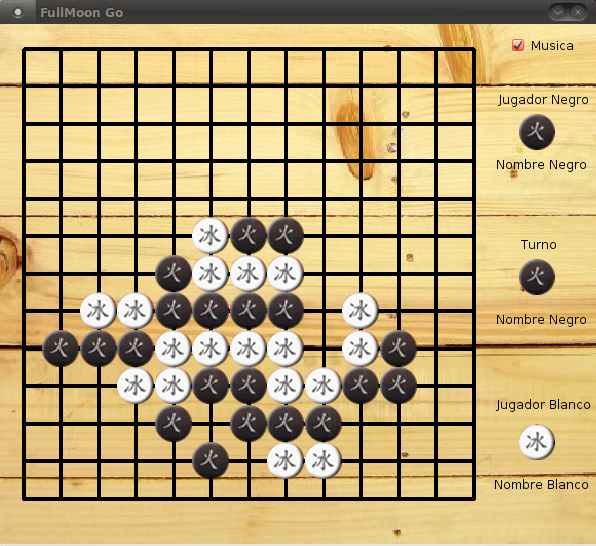
\includegraphics[scale=0.55]{./Diagramas/captura_tablero.png}
\end{center}

\newpage
\section{Evoluci\'on del Proyecto}

A continuaci\'on se detalla la evoluci\'on del proyecto a lo largo del cuatrimestre.

\begin{itemize}
 \item \textbf{11 de Marzo} Presentaci\'on en clase del Proyecto a Realizar
 \item \textbf{Semana 1 y 2} - An\'alisis del Go. \\
	Dado que la mayor\'ia de nosotros no conoc\'iamos el juego, durante las primeras semanas nos dedicamos aprender a jugar para 
	comprender la mec\'anica del juego y desarrollar estrategias eficientes m\'as adelante en el proyecto. 

  \item \textbf{Semana 3 y 4} - Reglas de Juego y an\'alisis de la soluci\'on\\
	Durante esta etapa analizamos la problem\'atica planteada y diagramamos la estructura general de la soluci\'on.\\
	Iniciamos con la implementaci\'on del tablero, el cual arma cadenas (o grupos) de piedras y valida las reglas del juego.

  \item \textbf{Semana 5 y 6} - Comienzo de interfaz gr\'afica\\
        Continuamos con el desarrollo del tablero y la creaci\'on de tests unitarios para validar su correcto funcionamiento.\\
	Comenzamos a desarrollar una interfaz gr\'afica para visualizar el tablero y poder empezar jugar ``player vs player''.

  \item \textbf{Semana 7 y 8} - Primeras Estrategias y Protocolo de Comunicaci\'on\\
	Comenzamos desarrollando estrategias simples (algunas de las cuales ahora quedaron como estrategias ``f\'aciles''). \\
	Seguimos con el desarrollo de la interfaz gr\'afica y empezamos a implementar el procesador de comandos de GTP, que es el protocolo de comunicaci\'on utilizado.

  \item \textbf{Semana 9 y 10} - Avance en Estrategias y Protocolo\\
	Agregamos la funcionalidad cliente/servidor para la implementaci\'on del protocolo GTP. \\
	Empezamos con el desarrollo de la estrategia MiniMax.

  \item \textbf{20 de Mayo} - Presentaci\'on de avances\\
	Mostramos la funcionalidad b\'asica del juego: partida ``player vs. player'' y ``player vs estrategia''
 
  \item \textbf{Semana 11} - Interfaz gr\'afica y Avance en estrategia\\
	Continuamos mejorando la estrategia MiniMax para que esta sea menos predecible y m\'as r\'apida al realizar una jugada.\\
	Creamos un men\'u de inicio para la selecci\'on del tama\~no del tablero y de la estrategia deseada para cada jugador.
  
  \item \textbf{Semana 12} - Juego Remoto\\
	Integramos la funcionalidad cliente/servidor a la aplicaci\'on para jugar partidas remotas contra engines de Go compatibles con
	el GNUgo en modo GTP.
  
  \item \textbf{Semana 13} - Avance en estrategia\\
	Desarrollamos una estrategia en base a MiniMax que llamamos ``MiniMax reducido'', la cual reduce el tiempo de c\'alculo considerablemente 
	durante las primeras jugadas al evaluar menor cantidad de jugadas posibles.

  \item \textbf{10 de Junio} - Presentaci\'on de avances\\
	Mostramos la aplicaci\'on jugando de forma remota y utilizando las estrategias MiniMax y MiniMax reducido.

  \item \textbf{Semana 14 y 15} - Detalles Finales\\
	Realizamos los ajustes finales, principalmente a la interfaz gr\'afica para mostrar informaci\'on del estado de la partida.
  
  \item \textbf{24 de Junio} - Presentaci\'on Final de la Aplicaci\'on - Cierre del Proyecto\\

\end{itemize}


\newpage

\section{Estrategias implementadas}
\label{sec-4.3}

   Actualmente se cuenta con cuatro estrategias de juego que serán
   utilizadas posteriormente para elaborar estrategias mas avanzadas:
\subsection{EstrategiaComputadoraAtacar}
\label{sec-4.3.1}

    Esta estrategia intenta ocupar casilleros adyacentes a las cadenas
    con menor grado de libertad del oponente, intentando capturarlas.
\subsection{EstrategiaComputadoraDefender}
\label{sec-4.3.2}

    Esta estrategia intenta ocupar casilleros adyacentes a las cadenas
    propias con menor grado de libertad, intentando evitar que sean
    capturadas.
\subsection{EstrategiaAtaqueCuidadoso}
\label{sec-4.3.3}

    Esta estrategia es una combinación de las estrategias
    ``EstrategiaComputadoraAtacar'' y
    ``EstrategiaComputadoraDefender''. Primero verifica que las
    cadenas propias no estén en peligro de ser capturadas. Si se
    encuentra una cadena propia en riesgo aplica la estrategia
    ``EstrategiaComputadoraDefender'', en caso contrario aplica
    ``EstrategiaComputadoraAtacar''.
\subsection{EstrategiaAtaqueCuidadosoMasInteligente}
\label{sec-4.3.4}

    Similar a la estrategia anterior, pero primero verifica si existe
    alguna cadena del oponente con grado de libertad 1. Si existe,
    verifica que ese grado de libertad no se deba a un ojo. Si no se
    deba a un ojo se procede a capturar al grupo. Si no se cumplen
    estas condiciones, se aplica la estrategia
    ``EstrategiaAtaqueCuidadoso''.

\subsection{EstrategiaMiniMax}

   Implementa una estrategia del tipo {\bf MiniMax}. En cada turno,
   arma una lista de todos los casilleros vac\'ios y despliega un
   \'arbol de jugadas por cada posible casillero. La profundidad hasta
   la cual despliega el \'arbol de jugadas es configurable. Al llegar a
   la profundidad deseada, se aplica la funci\'on de evaluaci\'on a
   los tableros resultantes.
   
   La funci\'on de evaluaci\'on tiene en cuenta las siguientes
   variables:
   
   \begin{itemize}
      \item Grados de libertad de MAX: Se cuentan todos los casilleros
        adyacentes a cada cadena de MAX libres (no se cuentan los
        repetidos). Se quiere que sea lo mayor posible.
      \item Cantidad de ojos de MAX
      \item Grados de libertad de la cadena mas corta de MAX: la
        variable a la que se le da m\'as importancia.
      \item Grados de libertad de la cadena mas corta de MIN.
      \item Grados de libertad de la cadena mas larga de MIN.
      \item Ojos de MIN.
   \end{itemize}
   
   Por encima de las variables arriba mencionadas, se encuentra la
   condici\'on de que alguna de alguna de las cadenas de MIN tenga
   grado 1. En ese caso se da por ganada la partida (en esa rama del
   \'arbol de jugadas).

   Al desplegar el \'arbol de jugadas, si en alg\'un nivel todos los
   movimientos son inv\'alidos, se da por finalizada la partida y no
   se sigue avanzando hasta los niveles mas profundos.

\subsection {MiniMax Reducido}

Se tienen en cuenta como jugadas posibles todos los
       casilleros libres del tablero. Se podr\'ia tener en cuenta
       solamente los casilleros adyacentes a todas las cadenas
       presentes en el tablero solamente, limitando as\'i las jugadas,
       pero reduciendo el procesamiento, eventualmente d\'andonos la
       posibilidad de descender un poco mas en el \'arbol de jugadas.

El MiniMax anteriormente explicado tiene en cuenta como jugadas posibles todos los casilleros libres del tablero. 
A diferencia de \'este, el MiniMax reducido solamente tiene en cuenta los casilleros adyacentes a las cadenas presentes en el tablero.
Si bien se limitan las posibles jugadas, se reduce el procesamiento logrando as\'i una respuesta m\'as r\'apida de la estrategia
(en particular en los primeros turnos que es cuando m\'as casilleros libres hay). Esta estrategia permitir\'ia descender a\'un m\'as en el 
\'arbol de jugadas.


\subsubsection{Mejoras posibles}

   La implementaci\'on MiniMax presentada se puede mejorar teniendo en
   cuenta lo siguiente:

   \begin{itemize}
     \item Si se es el primero en jugar, no es necesario descender en
       el \'arbol de jugadas. Ser\'ia conveniente comenzar con jugadas
       precalculadas.
     \item La cantidad de niveles que se baja en el \'arbol de jugadas
       es fija. Se puede parametrizar en funci\'on de las jugadas
       posibles. Al principio de la partida, al haber muchas
       posibilidades se elige por ejemplo descender hasta el nivel 3,
       pero a medida que quedan menos posibilidades (la mitad del
       tablero puede ser un caso) podr\'iamos aumentar un nivel sin
       perder mucha velocidad de respuesta.
     \item La funci\'on de evaluaci\'on actualmente es una suma pesada
       de diferentes variables. Se pueden implementar diferentes
       funciones de evaluaci\'on mas sofisticadas.
   \end{itemize}

\newpage
\section{Detalles de implementación}
\label{sec-4}

Estructura general de la soluci\'on:

\begin{center}
 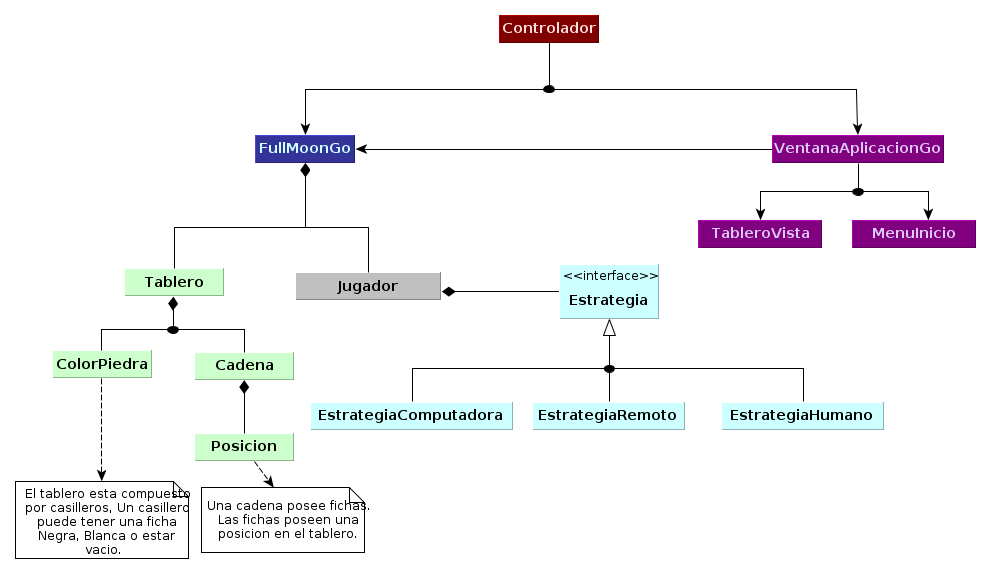
\includegraphics[scale=0.55]{./Diagramas/DiagramaClases/diagrama_de_clases.png}
\end{center}

La clase FullMoonGo posee la l\'ogica de control del juego, seleccionando al jugador correspondiente seg\'un el turno y
detectando el fin de la partida. El tablero es quien verifica la validez de una jugada, encapsulando toda la l\'ogica de cadenas y grados de libertad de una piedra.
Los jugadores ubica una piedra en el tablero, eligiendo su jugada en base a su estrategia asociada, la cual puede ser:
\begin{itemize}
 \item EstrategiaHumano\\
      Representa la jugada realizada por un humano mediante acciones con el mouse sobre la vista.
 \item EstrategiaRemota\\
      Obtiene la jugada realizada por un jugador conectado en red.
 \item	EstrategiaComputadora \\
      Aplica un algoritmo para decidir en qu\'e posici\'on del tablero jugar.
\end{itemize}

Por otro lado, el controlador interact\'ua con la vista, indic\'andole al modelo qu\'e estrategia asignar a cada jugador y
cu\'ando iniciar la partida. En cuanto a una partida remota, el controlador le indica al \'arbitro de la partida (quien maneja la interacci\'on 
con el usuario remoto) cuando crear una conexi\'on, ya sea como cliente o como servidor.

\subsection{Vista}
\label{sec-4.1}


Para implementar el aspecto visual de la aplicaci\'on se uso el la api de Java Swing. Principalmente se utilizaron las clases Frame como contenedor principal y Panel para las distintas pantallas. 
Estas son men\'u de inicio y  la vista del tablero.
En el men\'u se permite elegir la estrategia de cada jugador y se da la opci\'on de crear una partida como servidor o unirse a una partida remota como cliente.
En cuanto a la vista del tablero, \'esta muestra el estado actual del tablero. \\
La vista no posee l\'ogica alguna, sino que detr\'as de cada una hay un controlador que toma la informaci\'on y la utiliza seg\'un corresponda. 
De la misma forma, es el controlador quien espera cambios en el modelo para luego indicarle a la vista que debe actualizarse. Para implementar este mecanismo de comunicaci\'on de se utiliz\'o el patr\'on Observer provisto por la API de Java. Los subscritores son las clases de Control y las clases Observadas son las correspondientes al modelo.

Otro aspecto adicional de las clases de la vista es que manejan la reproducción de los sonidos de posicionamiento de piezas, siendo uno distinto para cada pieza. Para esto se uso la clase clip que resulta adecuada para una reproducci\'on repetida de sonidos cortos pues los mantiene cargados (En contraposicion a los Flujos de datos).

\subsection{Protocolo de comunicaciones}
\label{sec-4.2}
%  La clase remoto es la encargada del manejo del protocolo de texto Go(gtp), 
si el modelo desea enviar un mensaje lo debe hacer por esta clase. 
Como se puede observar en el diagrama servidor y cliente son hijos de remoto; 
esto se debe a que el proceso de mensajes entrantes y saliente es el mismo en ambos casos, 
la \'unica diferencia existente es el momento inicial donde se establece la conexi\'on. 
Para el proceso de los mensajes, tenemos dos cadenas de responsabilidades; una encargada de los mensajes respuestas
(los cuales se caracterizan por el inicio con el caracter \textbf{=}) y los mensajes comandos. 
Estas cadenas procesan dichos mensajes y le informan al modelo, para que el mismo decida como se debe continuar. \\
La versi\'on del protocolo utilizada es la 2, a pesar que el protocolo fue implementado totalmente; 
para los alcances del trabajo pr\'actico solo se utilizan los comandos m\'as importantes.

\begin{center}
 %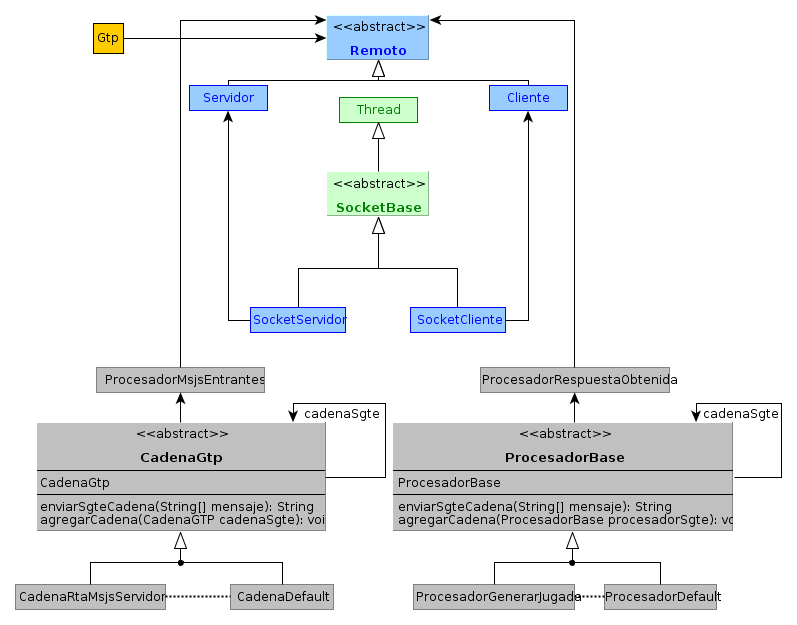
\includegraphics[width=500,height=500]{./Diagramas/DiagramaRemoto/diagrama_remoto.png}
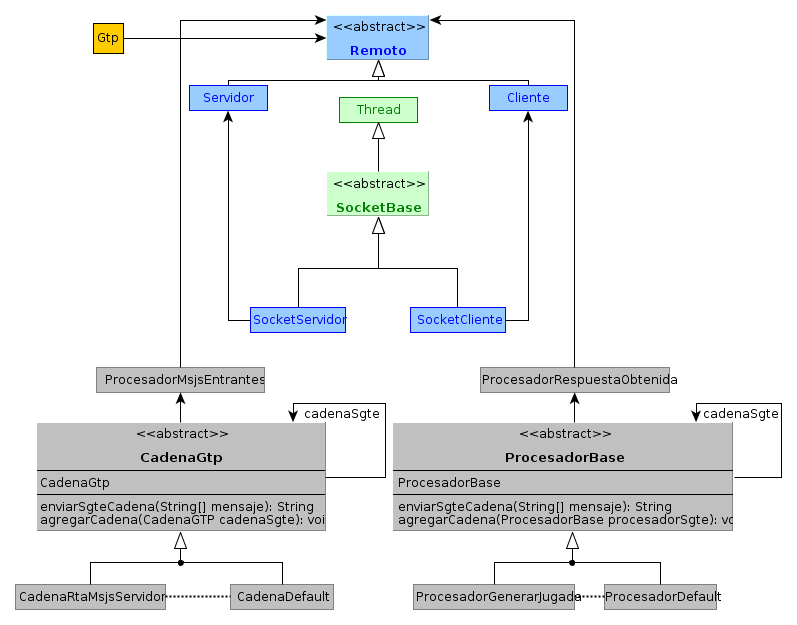
\includegraphics[scale=0.6]{./Diagramas/DiagramaRemoto/diagrama_remoto.png}
 % diagrama_remoto.png: 797x625 pixel, 72dpi, 28.12x22.05 cm, bb=0 0 797 625
\end{center}


La clase remoto es la encargada del manejo del protocolo de texto Go(gtp), 
si el modelo desea enviar un mensaje lo debe hacer por esta clase. 
Como se puede observar en el diagrama servidor y cliente son hijos de remoto; 
esto se debe a que el proceso de mensajes entrantes y saliente es el mismo en ambos casos, 
la \'unica diferencia existente es el momento inicial donde se establece la conexi\'on. 
Para el proceso de los mensajes, tenemos dos cadenas de responsabilidades; una encargada de los mensajes respuestas
(los cuales se caracterizan por el inicio con el caracter \textbf{=}) y los mensajes comandos. 
Estas cadenas procesan dichos mensajes y le informan al modelo, para que el mismo decida como se debe continuar. \\
La versi\'on del protocolo utilizada es la 2, a pesar que el protocolo fue implementado totalmente; 
para los alcances del trabajo pr\'actico solo se utilizan los comandos m\'as importantes.

\begin{center}
 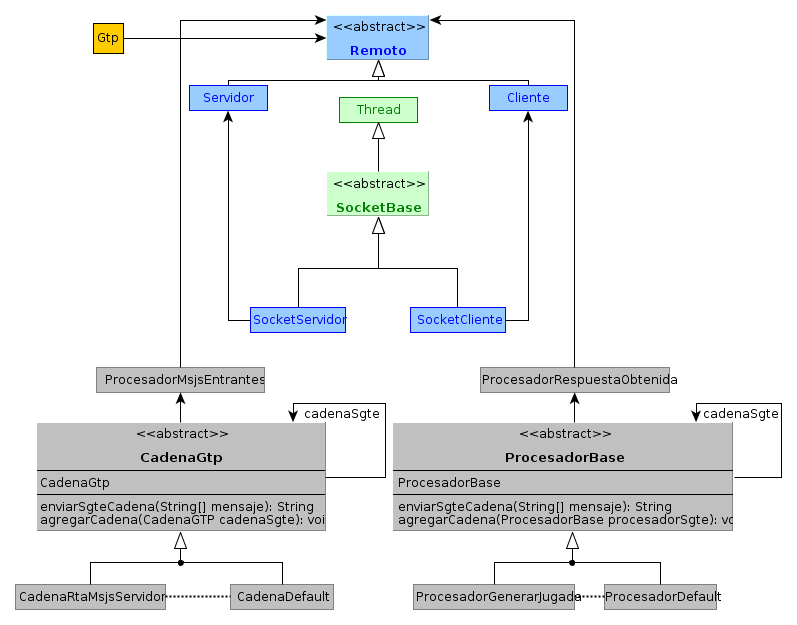
\includegraphics[scale=0.6]{./Diagramas/DiagramaRemoto/diagrama_remoto.png}
 \end{center}

\subsubsection{EstrategiaRemoto}
\label{sec-4.2.1}

  Para comunicar dos jugadores en red mediante el protocolo, se tiene una clase ``EstrategiaRemota'' la cual
abstrae al motor del juego del intercambio de mensajes entre jugadores. \\
Para notificar y pedir jugadas mediante el protocolo, 
se cuenta con una implementaci\'on que es compatible con el protocolo GTP para el GnuGo, el cual es un 
servidor pasivo que simplemente responde a los comandos enviados por GTP. Por esta raz\'on, implementamos
separadamente la estrategia remota para el servidor y para el cliente, para poder adaptarlos a los mensajes
que deben enviar y los que esperan recibir. \\ 
La convenci\'on de mensajes utilizada es la siguiente: 
\begin{itemize}
 \item EstrategiaRemotaCliente \\
      Se conecta con un servidor y determina el tama\~no del tablero mediante un mensaje \textit{``boardsize''.}\\
      En el turno del jugador remoto, se env\'ia la jugada realizada localmente mediante el mensaje \textit{``play''}, 
      luego se solicita la jugada al servidor remoto mediante un mensaje\textit{ ``genmove''} y se aguarda hasta recibir una respuesta. 
      Cuando esta respuesta llega, el jugador remoto puede poner la piedra recibida en el tablero. 
 \item EstrategiaRemotaServidor\\
      Crea un servidor remoto que espera la conexi\'on de un cliente. El primer mensaje debe ser un \textit{boardize} para determinar el tablero del juego.
      Dado que el servidor es pasivo, cuando es el turno del jugador remoto la estrategia espera la llegada de un mensaje \textit{``genmove'',} 
      el cual contesta con la \'ultima jugada local realizada. Luego, el servidor queda a la espera de la llegada de un mensaje 
     \textit{ ``play''} el cual indica la jugada remota a realizar.
  \item Fin Del Juego\\
      Al finalizar el juego (alguno de los dos jugadores gana), es el cliente quien env\'ia el mensaje de \textit{``quit''} para finalizar
      la comunicaci\'on mediante GTP.
  \item Desconexi\'on\\
      Ante una desconexi\'on repentina de alguno de los dos extremos, la partida finaliza mostrando un mensaje de empate.
\end{itemize}

A continuaci\'on se incluye un diagrama de secuencia describiendo la interacci\'on mencionada.

\begin{center}
 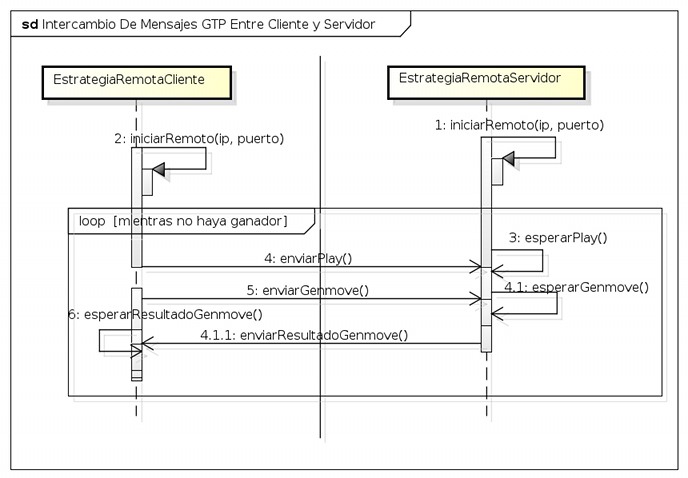
\includegraphics[scale=0.9]{./Diagramas/DiagramaRemoto/secuencia_estrategiaRemoto.png}
\end{center}

La estrategia remota realiza el intercambio de mensajes utilizando la implementaci\'on de la clase ``Remoto'' que corresponda (cliente o servidor).
Adem\'as, funciona como \'arbitro de la partida mediante GTP, coordinando los mensajes administrativos
como son el mensaje de salida (\textit{quit}) y el mensaje indicando el tablero (\textit{boardisze}).

\begin{center}
 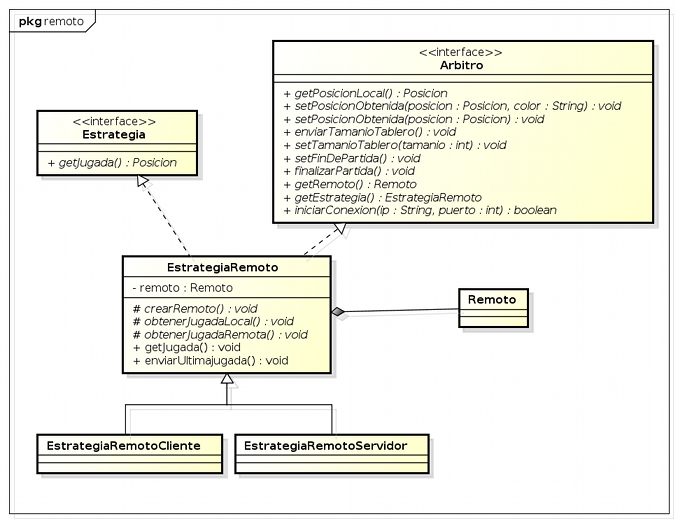
\includegraphics[scale=1.0]{./Diagramas/DiagramaRemoto/diagrama_estrategiaRemoto.png}
\end{center}

\newpage
\appendix
\section{Problemas y Soluciones}
A lo largo del proyecto nos encontramos con algunos inconvenientes a la hora de desarrollar la aplicaci\'on.

!!!!!!!!!!!!!!!!!!!1 Explicar!!!!!!!!!!!!!!

\end{document}
